

\title{Architectural Design Document}
\def \documentid {FLIGHTOS-UVIE-ADD-001}
\date{Issue 1.0, June 1, 2017}

\newcommand\affil[1]{\textsuperscript#1}

\def\preparedby {Armin Luntzer\affil{1}}
\def\checkedby {Roland Ottensamer\affil{1}, Christian Reimers\affil{1}}
\def\approvedby {Franz Kerschbaum\affil{1}}

\def\affiliations{
	\affil{1} Department of Astrophysics, University of Vienna
}

\documentclass{report}
%\usepackage[left = 2cm, right=2cm, top = 1cm]{geometry}
\usepackage[top = 2cm, bottom = 5cm]{geometry}

\usepackage[T1]{fontenc}
\usepackage{textcomp}

%\PassOptionsToPackage{table}{xcolor}


\usepackage{geometry}
\usepackage{fontspec}
%
\defaultfontfeatures[MyriadPro-SemiCondensed]{
	Path		= ../shared/fonts/,
	Extension	= .otf,
	UprightFont	= *-light,
	ItalicFont	= *-italic,
	BoldFont	= *-bold,
	BoldItalicFont	= *-bold-italic
%	LetterSpace	= 5pt		% Laufweite
}
%
\defaultfontfeatures[MyriadPro]{
	Path		= ../shared/fonts/,
	Extension	= .otf,
	UprightFont	= *-regular,
	ItalicFont	= *-italic,
	BoldFont	= *-bold,
	BoldItalicFont	= *-bold-italic
}%
\defaultfontfeatures[MyriadProLight]{
	Path		= ../shared/fonts/,
	Extension	= .otf,
	UprightFont	= MyriadPro-light,
	ItalicFont	= MyriadPro-light-italic,
}

\setmainfont{MyriadPro}



\makeatletter
\renewcommand\normalsize{%
\@setfontsize\normalsize{11pt}{14pt}
\abovedisplayskip 10\p@ \@plus2\p@ \@minus5\p@%
\abovedisplayshortskip \z@ \@plus2\p@%
\belowdisplayshortskip 5\p@ \@plus2\p@ \@minus3\p@%
\belowdisplayskip \abovedisplayskip%
\let\@listi\@listI%
}
\normalsize  
\makeatother



\usepackage{titlesec}

\titleformat{\chapter}[hang]
  {\fontspec{MyriadProLight}\fontsize{30}{36}\selectfont\color{uvie-blue}}
  {\fontspec{MyriadPro}\selectfont\thechapter.}{8pt}{}
\titlespacing*{\chapter}{0pt}{-20pt}{20pt}

\titleformat{\section}
  {\fontspec{MyriadPro}\fontsize{13}{16}\selectfont\color{uvie-blue}}
  {\thesection}{1em}{}

\titleformat{\subsection}
  {\fontspec{MyriadPro}\fontsize{13}{16}\selectfont\color{uvie-blue}}
  {\thesection}{1em}{}

\DeclareMathSizes{12}{55}{15}{15}

\usepackage[table]{xcolor}

% begin UVIE primary colours
\iffalse

% colours from numeric colour values in corporate design document
\definecolor{uvie-blue}{RGB}{0, 99, 166}
\definecolor{uvie-orangered}{RGB}{221, 72, 20}
\definecolor{uvie-goldenyellow}{RGB}{234, 171, 0}
% UVIE secondary colours
\definecolor{uvie-gray}{RGB}{102, 102, 102}
\definecolor{uvie-burgundy}{RGB}{167, 28, 73}

\else
% colours from actual colour samples in corporate design document
%r: 0 g:58 b:133
\definecolor{uvie-blue}{RGB}{0, 79, 150}
\definecolor{uvie-orangered}{RGB}{225, 55, 15}
\definecolor{uvie-goldenyellow}{RGB}{248, 169, 0}
% UVIE secondary colours
\definecolor{uvie-gray}{RGB}{104, 104, 104}
\definecolor{uvie-burgundy}{RGB}{141, 22, 51}

\fi
% end UVIE primary colours


% allowed UVIE logo height
\newlength{\maxlogoheight}\setlength{\maxlogoheight}{20mm}
\newlength{\medlogoheight}\setlength{\medlogoheight}{15mm}
\newlength{\minlogoheight}\setlength{\minlogoheight}{10mm}
%
% allowed space round logo: logoheight <= x <= 0.5 logoheight 
\def \maxlogospacing{1.0}
\def \medlogospacing{0.75}
\def \minlogospacing{0.5}

%
%elif \paperheight \equal {210mm} % A5
% todo: based on papersize: >= A4: 20mm, A5/long: 15mm, all smaller: 10mm
%\if \paperheight \equal {297mm}	  % A4
\newlength{\logoheight}{\setlength{\logoheight}{\maxlogoheight}
%elif \paperheight \equal {210mm} % A5
%\fi
%
% todo: pass as option
\newlength{\logospacing}{\setlength{\logospacing}{\medlogospacing\logoheight}


\newcommand{\fig}[1]{Figure \ref{#1}}


\newenvironment{keywords}%
   {\begin{trivlist}\item[]{\bfseries\sffamily Schlagworte:}\ }% oder "Keywords:"
   {\end{trivlist}}
%
\author{%
    Author 1 name \\
    Department name \\
    \texttt{email1@example.com}\vspace{40pt} \\
    Author 2 name \\
    Department name \\
    \texttt{email2@example.com}
    }


\usepackage{tabu}
\usepackage{colortbl}

\usepackage{array, ltxtable}
\usepackage[most]{tcolorbox}


\usepackage[some]{background}
\usepackage{tikz}
\backgroundsetup{
scale=1,
angle=0,
opacity=1,
placement=top,
contents={
	\begin{tikzpicture}[remember picture, blend mode = multiply]
		% field heights from top down: x | x | x/2 | remainder
		%
		\fill[white]		(-0.5\paperwidth,                 0.0)
							rectangle (0.5\paperwidth,       -3.0\logospacing);
		\fill[uvie-blue!75]	(-0.5\paperwidth,                -3.0\logospacing)
							rectangle (0.5\paperwidth, -2.0 * 3.0\logospacing);
		\fill[uvie-blue]	(-0.5\paperwidth,          -2.0 * 3.0\logospacing)
							rectangle (0.5\paperwidth, -2.5 * 3.0\logospacing);
		% mext can be image or colour, but must overlap with 3rd bar in multiply
		% blend mode
		% todo: make conditional on image option
		\fill[uvie-blue!75]	(-0.5\paperwidth,          -2.0 * 3.0\logospacing)
							rectangle (0.5\paperwidth,       -1.0\paperheight);
	\end{tikzpicture}}
}
%


\makeatletter
\let\doctitle\@title
\makeatother

\makeatletter
\let\docdatever\@date
\makeatother

\usepackage{fancyhdr}
\usepackage{lastpage}

\def\ifalogo{
\includegraphics[height = \medlogoheight]{../shared/images/uni_logo_astrophysik_cmyk.eps}}
\fancypagestyle{plain}{ % call style plain so it is used by chapter pages as well
	\fancyhf{}
	\fancyhead[R]{
		\fontspec{MyriadPro}\docdatever \\
		\vspace{2em}
		Page \thepage\ of \pageref*{LastPage} 
	}

	\fancyhead[C]{
		{
			\fontspec{MyriadPro}
			\documentid \\
			\vspace{.7em}
			\doctitle
			\vspace{.9em}
		}
	}
	\fancyhead[L]{
		\ifalogo%
	}
}
\setlength\headheight{80pt}
\pagestyle{plain}


% def \preparedby, \checkedby, \approvedby, \documentid, \docdatever, \doctitle
\def\approvalpage{
	\clearpage
	\pagestyle{empty}
	\null
	\vfil

	{\fontspec{MyriadPro}\fontsize{20}{24}\selectfont\color{uvie-blue}
	 \doctitle}

	\vspace*{1\baselineskip}

	\begin{tabular}{@{}ll}
		\textbf{Reference:}   & \documentid \\[2ex]
		\textbf{Version:}     & \docdatever \\[6ex]
		\textbf{Prepared by:} & \preparedby \\[1ex]
		\textbf{Checked by:}  & \checkedby  \\[1ex]
		\textbf{Approved by:} & \approvedby \\[1ex]
	\end{tabular}

	\vspace*{0.5\baselineskip}
	{\footnotesize \affiliations}


	\vfill

	\begin{minipage}[b]{0.9\textwidth}
	\footnotesize\raggedright
	\setlength{\parskip}{0.5\baselineskip}
	Copyright \copyright \the\year\ \par
	Permission is granted to copy, distribute and\slash or modify this
	document under the terms of the GNU Free Documentation License,
	Version 1.3 or any later version published by the Free Software
	Foundation; with no Front-Cover, no Logos of the University of Vienna.
	\end{minipage}
	\vspace*{2\baselineskip}
	\cleardoublepage

	\pagestyle{plain}
}

\newcommand{\uvietitlepage}[3]{%
\begin{titlepage}
\BgThispage
%
%
\begin{tikzpicture}[overlay, remember picture]
\node[anchor	= north west,
      xshift	= \logospacing,
      yshift	=-\logospacing] 
      at (current page.north west)
     {
\includegraphics[height = \logoheight]{../shared/images/uni_logo_astrophysik_cmyk.eps}}; 
\end{tikzpicture}
%
\begin{tikzpicture}[overlay, remember picture]
\node[anchor	= north east,
      xshift	=-\logospacing,
      yshift	=-\logospacing] 
      at (current page.north east)
     {
\includegraphics[height = \logoheight]{../shared/images/uni_logo_farbe_02.eps}}; 
\end{tikzpicture}
%
%
%
% main title, must not exceed 3 lines 
\begin{tikzpicture}[overlay, remember picture]
\node[anchor			= north west,
      xshift			= \logospacing,
      yshift			=-\logospacing * 3.0,
	  minimum height	= \logospacing * 3.0,
	  text width		= \textwidth]
      at (current page.north west)
      {\fontsize{30pt}{36pt}\selectfont
       \textcolor{white}
       {
			\uppercase{#1}
       }
       \par
      };
\end{tikzpicture}
%
% subtitle, must not exceed 3 lines 
\begin{tikzpicture}[overlay, remember picture]
\node[anchor			= north west,
      xshift			= \logospacing,
      yshift			=-\logospacing * 5.5,
	  minimum height	= \logospacing * 2.5,
	  text width		= \textwidth]
      at (current page.north west)
      {\fontsize{13pt}{16pt}\selectfont
       \textcolor{white}
       {
			\uppercase{\textbf {#2}}
       }
       \par
      };
\end{tikzpicture}
%
%\noindent
%\hfill
% \hspace*{-3cm}
\begin{tikzpicture}[overlay, remember picture]
\node[anchor=south east,		%anchor is upper left corner of the graphic
      xshift  = 0.5cm,		%shifting around
      yshift  = -0.5cm] 
     	at (current page.south east) %left upper corner of the page
     {\includegraphics[width=14.0cm]{#3}}; 
\end{tikzpicture}
%
%
\end{titlepage}
%
\restoregeometry
%
\newpage
}% newcommand uvietitlepage


\usepackage{xintexpr, xinttools}

\usepackage{xr-hyper} % load before hyperref
\usepackage{hyperref}% check if ok with hyperlinks
\hypersetup{colorlinks=true, linkcolor=uvie-blue}

\usepackage{xifthen}
\usepackage{pifont}
\usepackage{adjustbox}	% \rot

\usepackage{stringstrings}


\newcommand{\requirements}{}
\newcommand{\designs}{}
\providecommand*\phantomsection{}

\makeatletter

\newcommand{\req}[1]{%
	\textbf{R-#1}%
	\phantomsection
	\def\@currentlabel{R-#1}%
	\label{req@#1}%
  	\@ifundefined {req@#1} {%
  		\global\@namedef{req@#1}{}%
  		\g@addto@macro\requirements{{req@#1}}%
	}{}%
}

\newcommand{\reqgoal}[1]{%
	\textbf{G-#1}%
	\phantomsection
	\def\@currentlabel{G-#1}%
	\label{req@#1}%
	\@ifundefined {req@#1} {%
		\global\@namedef{req@#1}{}%
		\g@addto@macro\requirements{{req@#1}}%
	}{}%
}

\newcommand{\meetsthisreq}[1]{% (renamed from \meetsreq above)
  \@ifundefined {req@#1@ismetby} {%
  \global\@namedef{req@#1@ismetby}{}%
  }{}% this is called multiple times when creating a table, generate only one
  \ref{REQ-req@#1}%
  \expandafter\g@addto@macro\csname req@#1@ismetby\expandafter\endcsname 
              \expandafter {\expandafter{\@currentdesign}}%
}

\newcommand{\meetsreq}[1]{% (handles comma separated list)
  \xintListWithSep{, }{\xintApply{ \meetsthisreq}{\xintCSVtoList{#1}}}%
}



\newcommand{\designswithreq}[1]% 
% The space before \ref below is intentional and will be swallowed by \xintApply
% It is not mandatory however, the thing works without it too.
 {\csname #1@ismetby\endcsname}

\newcommand{\designswithreqref}[1]% 
% The space before \ref below is intentional and will be swallowed by \xintApply
% It is not mandatory however, the thing works without it too.
 {\xintListWithSep{, }{\xintApply { \ref}{\csname #1@ismetby\endcsname }}}

\newcommand{\newdesign}[1]{%
  	\textbf{D-#1}%
  	\phantomsection
  	\def\@currentlabel{D-#1}%
	\label{design@#1}%
  	\@ifundefined {design@#1} {%
  		\global\@namedef{design@#1}{}%
		\gdef\@currentdesign{design@#1}%
  	\g@addto@macro\designs{{design@#1}}%
	}{}
}


\newcommand{\design}[5]{%
	\rowcolors{1}{white}{white}%
	\begin{tcolorbox}[enhanced, notitle, clip upper,%
			  sharp corners, colframe = white, colback = white,%
		tabularx={%
						  p{0.15\columnwidth}%
				>{\arraybackslash\raggedright}p{0.10\columnwidth}%
				>{\arraybackslash}X%
			}%
		]%
	%
	\vspace{-.65\baselineskip}	% uuuaaahhh..why? :(
	\cellcolor{uvie-blue!75}\color{white}\newdesign{#1} &%
	\vspace{-.65\baselineskip}%
	\cellcolor{uvie-blue!50}\color{white}\textbf{Identifier} &%
	\vspace{-.65\baselineskip}%
	\cellcolor{uvie-blue!50}\color{white}\textbf{Function} \\%
	& #2 & #3%

	\\%
	\vspace{-1em}%
	\arrayrulecolor{uvie-blue!75}\renewcommand{\arraystretch}{1.2}
	\color{uvie-blue!75}\textbf{Purpose} &%
	\multicolumn{2}{|>{\arraybackslash\raggedright}X}{#4}%

	\ifthenelse{\isempty{#5}} {}{%
		\\%
		\vspace{-1em}%
		\arrayrulecolor{uvie-blue!75}\renewcommand{\arraystretch}{1.2}
		\color{uvie-blue!75}\textbf{Comment} &%
		\multicolumn{2}{|>{\arraybackslash}X}{#5}%
	}%
	\vspace{1em}
	\end{tcolorbox}%
}





\newcommand{\requirement}[4]{%
	\rowcolors{1}{white}{white}%
	\begin{tcolorbox}[enhanced, notitle, clip upper,%
			  sharp corners, colframe = white, colback = white,%
		tabularx={%
						  p{0.15\columnwidth}%
				>{\arraybackslash\raggedright}p{0.15\columnwidth}%
				>{\arraybackslash}X%
			}%
		]%
	%
	\vspace{-.65\baselineskip}	% uuuaaahhh..why? :(
	\cellcolor{uvie-blue!75}\color{white}\req{#1} &%
	\vspace{-.65\baselineskip}%
	\cellcolor{uvie-blue!50}\color{white}\textbf{Short Text} &%
	\vspace{-.65\baselineskip}%
	\cellcolor{uvie-blue!50}\color{white}\textbf{Software Requirement} \\%
	& #2 & #3%

	\ifthenelse{\isempty{#4}} {}{%
		\\%
		\vspace{-1em}%
		\arrayrulecolor{uvie-blue!75}\renewcommand{\arraystretch}{1.2}%
		\color{uvie-blue!75}\textbf{Comment}&%
		\multicolumn{2}{|>{\arraybackslash}X}{#4}%
	}%
	\vspace{1em}
	\end{tcolorbox}%
}



\newcommand{\goal}[4]{%
	\rowcolors{1}{white}{white}%
	\begin{tcolorbox}[enhanced, notitle, clip upper,%
			  sharp corners, colframe = white, colback = white,%
		tabularx={%
						  p{0.15\columnwidth}%
				>{\arraybackslash}p{0.2\columnwidth}%
				>{\arraybackslash}X%
			}%
		]%
	%
	\vspace{-.65\baselineskip}	% uuuaaahhh..why? :(
	\cellcolor{uvie-gray!75}\color{white}\reqgoal{#1} &%
	\vspace{-.65\baselineskip}%
	\cellcolor{uvie-gray!50}\color{white}\textbf{Short Text} &%
	\vspace{-.65\baselineskip}%
	\cellcolor{uvie-gray!50}\color{white}\textbf{Software Requirement} \\%
	& #2 & #3%
	\ifthenelse{\isempty{#4}} {}{%
		\\%
		\vspace{-1em}%
		\arrayrulecolor{uvie-gray!75}\renewcommand{\arraystretch}{1.2}
		\color{uvie-gray!75}\textbf{Comment} &%
		\multicolumn{2}{|>{\arraybackslash}X}{#4}%
	}%
	\vspace{1em}
	\end{tcolorbox}%
}





\newcommand{\exportrequirements}{%
\AtEndDocument{%
	\newwrite\reqfile
	\immediate\openout\reqfile=requirements.list
	\immediate\write\reqfile{\string\renewcommand{\string\requirements}{\requirements}}
	\immediate\closeout\reqfile
}}%


\makeatletter


\newcommand*\traceabilitymatrix[]{%
%
	\newcommand{\numitems}[1]{{\expandafter\xintLength\expandafter{##1}}}%
	\newcommand*\OK{\ding{51}}%
%
	\newcounter{numdesigns}%
	\setcounter{numdesigns}{\numitems{\designs}}%
	\stepcounter{numdesigns}%
%
	\newcommand*\rot{\multicolumn{1}{R{90}{0em}}}%
%
	%\begin{table}[h]
	\newcolumntype{C}{>{\centering\arraybackslash} m{0.2cm}}%
	\newcolumntype{R}[2]{>{\adjustbox{angle=##1,lap=\width-(##2)}\bgroup}l<{\egroup}}%
	\rowcolors{1}{uvie-gray!25}{white}%
	\begin{longtable}{c*{\value{numdesigns}}CC} %+1 linespacing column
	\xintFor* ##1 in \designs \do {%
		&  \rot{\fontspec{MyriadPro}\fontsize{8}{9}\ref{##1}\,\,\normalfont}%
	} \\%
	\endhead
	% it's hilariously inefficient, faster methods are welcome...
	\xintFor* ##1 in \requirements \do {%
	% TODO: recolor link if goal
	%	\isnextbyte[q]{R}{\string\ref{##1}} \par
	%	\if T\theresult moopp\hypersetup{filecolor=uvie-burgundy}\fi

		\fontspec{MyriadPro}\fontsize{8}{9}\ref{REQ-##1}\normalfont %
		\hypersetup{filecolor=uvie-blue}
		\xintFor* ##2 in \designs \do {%
			&%
			\xintFor* ##3 in {\designswithreq{##1}} \do {%
				\ifthenelse{\equal{##2}{##3}} {%
					\cellcolor{uvie-blue!50}%
					%\OK
					\xintBreakFor%
				}{}%
			}%
		}\\[0.1cm]%
	}%
	\end{longtable}%
	%\end{table}%
}%


\usepackage{stringstrings}

\def\rereadauxdesignlabels{
	\newtoks\designlist%
	\newread\zz%
	\immediate\openin\zz=\jobname.aux%
	\loop%
	\ifeof\zz\else%
	\read\zz to \tmp%
	\expandafter\findlabeldesign\tmp\relax\findlabel%
	\repeat%
}


\long\def\findlabeldesign#1#2\findlabel{%
 \ifx\newlabel#1\designlist\expandafter{\the\designlist\showlabeldesign#2}\fi}


%hyperref has 4 felds in each label could use them but don't here
\def\showlabeldesign#1#2{%
	%\begin{minipage}{\textwidth}%
	\findwords[q]{\expandafter\string\detokenize{#1}}{design}%
		\ifnum\theresult>0%
		\par\noindent\ref{#1}\dotfill\pageref{#1}%
		\fi%
	%\end{minipage}%
}


\def\rereadauxrequirementlabels{
	\newtoks\requirementlist
	\newread\zz
	\immediate\openin\zz=\jobname.aux
	\loop
	\ifeof\zz\else
	\read\zz to \tmp
	\expandafter\findlabelrequirement\tmp\relax\findlabel
	\repeat
}


\long\def\findlabelrequirement#1#2\findlabel{%
 \ifx\newlabel#1\requirementlist\expandafter{\the\requirementlist\showlabelrequirement#2}\fi}

\newsavebox{\fminipagebox}
\NewDocumentEnvironment{fminipage}{m O{\fboxsep}}
 {\par\kern#2\noindent\begin{lrbox}{\fminipagebox}
  \begin{minipage}{#1}\ignorespaces}
 {\end{minipage}\end{lrbox}%
  \makebox[#1]{%
    \kern\dimexpr-\fboxsep-\fboxrule\relax
    \fbox{\usebox{\fminipagebox}}%
    \kern\dimexpr-\fboxsep-\fboxrule\relax
  }\par\kern#2
 }


%hyperref has 4 felds in each label could use them but don't here
\def\showlabelrequirement#1#2{%
	\begin{minipage}{\textwidth}%
	\findwords[q]{\expandafter\string\detokenize{#1}}{req}%
		\ifnum\theresult>0%
		\par\noindent\ref{#1}\dotfill\pageref{#1}%
		\fi%
	\end{minipage}%
}

\usepackage[xindy, nopostdot, numberedsection, style=super, section, toc, acronyms, nogroupskip]{glossaries}
\usepackage{xparse}

\setlength{\glsdescwidth}{0.8\textwidth}
\renewcommand{\glsnamefont}[1]{\textbf{#1}}

% label, acronym, name, description
\DeclareDocumentCommand{\newdualentry}{ m m m m } {
	\newglossaryentry{gls-#1}{
	name={#3 (\gls{#1})},
	description={#4}, nonumberlist
	}
	\newglossaryentry{#1}{
		type=\acronymtype,
		name={#2},
		first={#3 (#2)},
		firstplural={#3s (#2s)},
		see={[Glossary:]{\gls{gls-#1}}},
		description=\glslink{gls-#1}{#3},
		nonumberlist
	}%
}
%%% \gls{ABBREV} to point at Acronym/Abbreviation index
%%% \gls{gls-ABBREV} to point to glossary


\newdualentry{ADC}%
  {ADC}%
  {Analog to Digital Converter}%
  {An Analog to Digital Converter is a system that converts an analog signal
   into a quantized digital signal. Its counterpart is the \gls{DAC}.}%

\newdualentry{API}%
  {API}%
  {Application Programming Interface}%
  {The Application Programming Interface defines how a developer can write
   a program that requests services from an operating system or application.
   \glspl{API} are implemented by function calls composed of verbs and nouns,
   i.e. a function to execute on an object.}%

\newdualentry{BSP}%
  {BSP}%
  {Board Support Package}%
  {A Board Support Package is the implementation of a specific interface defined
   by the abstract layer of an operating system that enables the latter to run
   on the particular hardware platform.}%

\newdualentry{CPU}%
  {CPU}%
  {Central Processing Unit}%
  {The Central Processing Unit is the electronic circuitry that interprets
  instructions of a computer program and performs control logic, arithmetic,
  and input/output operations specified by the instructions. It maintains
  high-level control of peripheral components, such as memory and other devices.}%

\newdualentry{DAC}%
  {DAC}%
  {Digital to Analog Converter}%
  {A Digital to Analog Converter is a system that converts a quantized digital
   signal into an analog signal. Its counterpart is the \gls{ADC}.}%

\newdualentry{DMA}%
  {DMA}%
  {Direct Memory Access}%
  {Direct Memory Access is a feature of a computer system that allows hardware
   subsystems to access main system \gls{gls-RAM} directly, thereby bypassing
   the \gls{gls-CPU}.}%

\newdualentry{DSP}%
  {DSP}%
  {Digital Signal Processor}%
  {A Digital Signal Processor is a specialised processor with its architecture %
   targeting the operational needs of digital signal processing.}%

\newdualentry{ELF}%
  {ELF}%
  {Executable and Linkable Format}%
  {The Executable and Linkable Format is a common standard file format for
   executables, object code, shared libraries, and core dumps.}%

\newdualentry{FIFO}%
  {FIFO}%
  {First In - First Out}%
  {In FIFO processing, the "head" element of a queue is processed first.
   Once complete, the element is removed and the next element in line becomes
   the new queue head.}%

\newdualentry{FPU}%
  {FPU}%
  {Floating Point Unit}%
  {A co-processor unit that specialises in floating-point calculations.}%

\newdualentry{ILP}%
  {ILP}%
  {Instruction Level Parallelism}%
  {Instruction-level parallelism (ILP) is a measure of how many instructions in
   a computer program can be executed simultaneously by the \gls{CPU}.}%

\newdualentry{ISR}%
  {ISR}%
  {Interrupt Service Routine}%
  {An Interrupt Service Routine is a function that handles the actions needed
   to service an interrupt.}%

\newdualentry{GCC}%
  {GCC}%
  {GNU Compiler Collection}%
  {The GNU Compiler Collection is a compiler system produced by the
   GNU project. It is part of the GNU toolchain collection of programming
   tools.}%

\newglossaryentry{GNU}{
  name={GNU},
  description={GNU is a recursive acronym that stands for "GNU's Not Unix!".
	      The GNU project is a free software collaboration project announced
	      in 1987. Users are free to run GNU-licensed software, share, copy,
	      distribute, study and modify it. GNU software guarantees these
	      freedom-rights legally via its license and is thefore free
      	      software.},
  nonumberlist
}

\newglossaryentry{LEON2}{
  name={LEON2},
  description={The LEON2 is a synthesisable VHDL model of a 32-bit processor
	       compliant with the SPARC V8 architecture. It is highly
	       configurable and particularly suitable for \gls{SoC} designs.
	       Its source code is available under the GNU LGPL license},
  nonumberlist
  }

\newglossaryentry{LEON3}{
  name={LEON3},
  description={The LEON3 is an updated version of the \gls{LEON2}, changes
	       include \gls{gls-SMP} support and a deeper instruction pipeline},
  nonumberlist
  }

\newglossaryentry{LEON3-FT}{
  name={LEON3-FT},
  description={The LEON3-FT is a fault-tolerant version of the \gls{LEON3}.
  	       Changes to the base version include autonomous error handling,
       	       cache locking and different cache replacement strategies.},
  nonumberlist
  }

\newdualentry{MMU}%
  {MMU}%
  {Memory Management Unit}%
  {A Memory Management Unit performs address space translation between physical
   and virtual memory pages and protects unprivileged access to certain memory
   regions.}%

\newdualentry{MPPB}%
  {MPPB}%
  {Massively Parallel Processor Breadboarding system}%
  {The Massively Parallel Processor Breadboarding system is a proof-of-concept %
   design for a space-hardened, fault-tolerant multi-DSP system with various %
   subsystems to build a powerful digital signal processing system with a high %
   data throughput. Its distinguishing features are the \gls{gls-NoC} and the
   \gls{Xentium} \glspl{DSP} controlled by a \gls{LEON2} processor.
   It was developed under ESA contract 21986 by Recore Systems B.V.}%

\newdualentry{NGAPP}%
  {NGAPP}%
  {Next Generation Astronomy Processing Platform}%
  {Next Generation Astronomy Processing Platform was an evaluation of the
   \gls{MPPB} performed in a joint effort of RUAG Space Austria and the
   Department of Astrophysics of the University of Vienna.
   The project was funded under ESA contract 40000107815/13/NL/EL/f.}%

\newdualentry{NoC}%
  {NoC}%
  {Network On Chip}%
  {A Network On Chip is a communication system on an integrated circuit that
   applies (packet based) networking to on-chip communication. It offers
   improvements over more conventional bus interconnects and is more scalable
   and power efficient in complex \gls{gls-SoC} desgins.}%

\newdualentry{POSIX}
  {POSIX}
  {Portable Operating System Interface}
  {The Portable Operating System Interface is a family of standards specified
   by the IEEE Computer Society for maintaining compatibility between
   operating systems.}%

\newdualentry{PUS}
  {PUS}
  {Packet Utilisation Standard}
  {The Packet Utilisation Standard addresses the end-to-end transport of telemetry
   and telecommand data between user applications on the ground and applications
   onboard a satellite. See also ECSS-E-70-41A.}%

\newdualentry{RAM}%
  {RAM}%
  {Random-Access Memory}%
  {Random-Access Memory is a type of memory where each memory cell may be
   accessed directly via their memory addresses.}%

\newdualentry{RISC}%
  {RISC}%
  {Reduced Instruction Set Computing}%
  {RISC is a \gls{CPU} design strategy that intends to improve performance by
   combining a simplified instruction set with a microprocessor architecture
   that is capable of executing an instruction in a smaller number of clock
   cycles.}%

\newdualentry{RMAP}%
  {RMAP}%
  {Remote Memory Access Protocol}%
  {The Remote Memory Access Protocol is a form of \gls{SpaceWire} communication
   that transparently communicates writes to memory mapped regions between
   different hardware devices.}%


\newdualentry{RR}%
  {RR}%
  {Round Robin}%
  {Round Robin is a scheduling algorithm where time slices are assigned in equal
   poritions and in circular order. In the context of threads, priorities are
   usually only used to control re-scheduling order when a mutex is accessed by
   a thread.}%

\newacronym{RSA}{RSA}{RUAG Space Austria}

\newdualentry{SMP}%
  {SMP}%
  {Symmetric Multiprocessing}%
  {Symmetric Multiprocessing denotes computer architectures, where two or more
   identical processors are connected to the same periphery and are controlled
   by the same operating system instance.}%

\newdualentry{SoC}%
  {SoC}%
  {System On Chip}%
  {A System On Chip is an integrated circuit that combines all components of a %
   computer or other electronic system into a single chip.}%

\newglossaryentry{SpaceWire}{
  name={SpaceWire},
  description={SpaceWire is a spacecraft communication network based in part
               on the IEEE 1355 standard of communications.},
  nonumberlist
  }

\newglossaryentry{SPARC}{
  name={SPARC},
  description={SPARC ("scalable processor architecture") is a \gls{gls-RISC}
  	       instruction set architecture developed by Sun Microsystems in
	       the 1980s. The distinct feature of SPARC processors is the high
	       number of \gls{gls-CPU} registers that are accessed similarly to
	       stack variables via ``sliding windows''.},
  nonumberlist
  }

\newdualentry{SSDP} % label
  {SSDP}            % abbreviation
  {Scalable Sensor Data Processor}  % long form
  {The Scalable Sensor Data Processor (SSDP) is a next generation on-board %
   data processing mixed-signal ASIC, envisaged to be used in future scientific %
   payloads requiring high-performance on-board processing capabilities. %
   It is built opon a heterogeneous multicore architecture, combining two %
   \gls{Xentium} \gls{DSP} cores with a general-purpose \gls{LEON3-FT} control %
   processor in a \gls{gls-NoC}.} % description


\newdualentry{TCM}%
  {TCM}%
  {Tightly-Coupled Memory}%
  {Tightly-Coupled Memory is the local data memory that is directly accessible %
   by a Xentium's load/store unit. It can be viewed as a completely %
   program-controlled data cache.}%


\newacronym{UVIE}{UVIE}{University of Vienna}

\newdualentry{VLIW}%
  {VLIW}%
  {Very Long Instruction Word}%
  {Very Long Instruction Word is a processor architecture design concept that
   exploits \gls{gls-ILP}. This approach allows higher performance at a smaller
   silicone footprint compared to serialised instruction processors, as no
   instruction re-ordering logic to exploit superscalar capabilities of the
   processor must be integrated on the chip, but requires either code to be
   tuned manually or a very sophisticated compiler to exploit the full potential
   of the processor.}%

\newglossaryentry{Xentium}{
  name={Xentium},
  description={The Xentium is a high performance \gls{gls-VLIW} \gls{DSP} core.
               It operates 10 parallel execution slots supporting 32/40 bit
	       scalar and two 16-bit element vector operations.},
  nonumberlist
  }


% do not remove
\glsresetall
\makeglossaries


\usepackage{vhistory}

\usepackage{biblatex}
\addbibresource{../shared/bibliography.bib}


\externaldocument[REQ-]{../requirements/software_requirements}
\input{../requirements/requirements.list}


\rereadauxdesignlabels


\begin{document}


\setmainfont{MyriadPro-SemiCondensed}
\uvietitlepage%
{Lean OS --\\ An operating system for the SSDP}%
{\doctitle}%
{../shared/images/logo2.pdf}
\setmainfont{MyriadPro}

\approvalpage

\tableofcontents
\newpage


\chapter*{List of Designs}
\the\designlist


\begin{versionhistory}
  \vhEntry{0.0}{30.09.2015}{AL}{draft architecture created based on \gls{NGAPP}}
  \vhEntry{0.1}{16.03.2016}{AL}{initial version with updated specifications from \gls{MPPB}v2}
  \vhEntry{0.2}{02.05.2016}{AL}{revised after internal design review}
  \vhEntry{1.0}{01.06.2017}{FK}{document approved}
\end{versionhistory}


\chapter{Introduction}

\section{Purpose of the Document}

This document specifies the software architecture for the operating system
kernel FlightOS. This document targets developers, testers and advanced users of
FlightOS. It is assumed that the reader is familiar with the user requirements
and/or the software user manual. \\


\noindent
This document follows the document structure for software design documents 
found in Annex F of ECSS-E-ST-40C \cite{ECSS40C}.


\section{Scope of the Software}

The architectural design aims to be at a high degree of encapsulation, with a
comparatively restricted number of system call interfaces to user space.
The user \gls{API} of FlightOS will orient itself to \gls{POSIX} standards where
applicable. Extra functionality that is typically found in supporting
C libraries is part of the user space and must be implemented accordingly.



\chapter{Applicable and Reference Documents} % does not break automatically for some reason

\printbibliography[heading=none]


\chapter{Terms, Definitions and Abbreviated Items}

\printglossary[type=acronym]
\printglossary[type=main, style=altlist]


\chapter{Software Design Overview}



\section{Software Static Architecture}

\begin{figure}[htb]
\begin{center}
	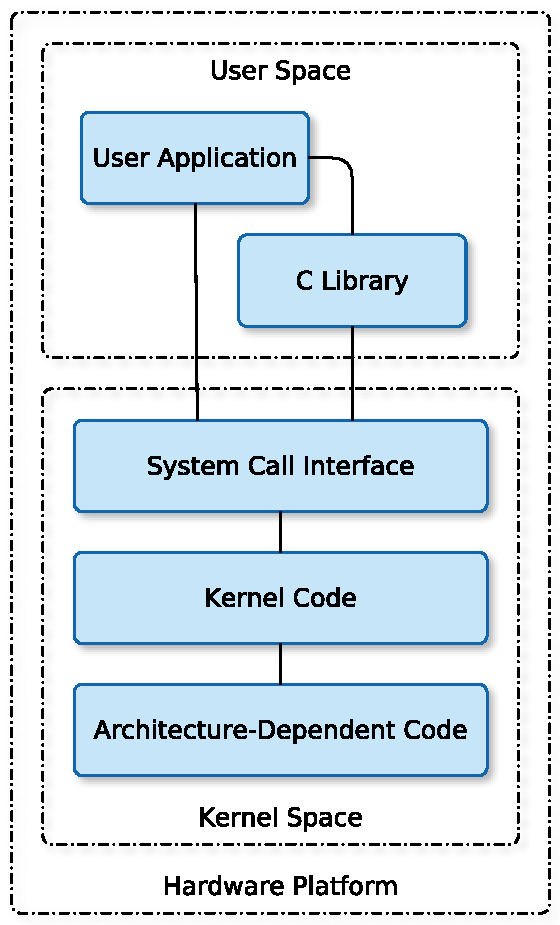
\includegraphics[width=0.4\columnwidth]{images/OS_fundamental_architecture}
	\caption{The fundamental architecture of FlightOS}
	\label{fig:fundamental_architecture}
\end{center}
\end{figure}

The fundamental architecture of FlightOS is shown in
\fig{fig:fundamental_architecture}. At the top is the user space, where user
applications are set up and executed. The C library is part of the user space.
It provides the system call interface that connects the user to kernel space
functionality and memory address space. Below the user space is the kernel
space. Here, the tasks of the operating system kernel are executed.

Kernel space can be further divided into three gross layers. At the top is the
system call interface, which implements any I/O functionality to the user space.
Below the system call interface is the architecture-independent kernel code.
While FlightOS is not designed with a high degree of portability in mind, it is
nonetheless sensible not to mix hardware dependent code into layers that run
on abstract functional concepts. On the lowest level sits the
architecture-dependent code, which forms what is typically called a \gls{BSP}.
This code serves as platform-specific glue to the underlying hardware.


\section{Software Dynamic Architecture}

FlightOS itself has no real time requirements. It does offer real time support for
threads in both kernel and user space, these are however specific to the
implementation of user space code or drivers/modules.

\section{Software Behaviour}

The behaviour of FlightOS is configuration-dependent. Usually, the kernel will
configure itself and the hardware, followed by user space initialisation.

Without user space, all actions by the drivers or other subcomponents will be
their default action in base configuration. To give an example, interface
drivers will usually ignore their inputs and drop all received.




\section{Interfaces Context}

The internal and external software interfaces of FlightOS are described as part
of its source code in Doxygen markup, from which a document can be generated.

\section{Long Lifetime Software}

FlightOS is designed with the \gls{SSDP} as a target platform. To allow re-use
and adaptation to new hardware, the software components of FlightOS are designed
to be modular. Unless neeeded for particular drivers, all hardware access is
abstracted into a separate layer as much as possible, so improved portability
is ensured.


\section{Memory and CPU Budget}

FlightOS is designed to work within the constraints of the \gls{SSDP} hardware
specification. Care is taken to minimise overheads, but run time needs of the
user ultimately define memory and CPU usage of the operating system.


\section{Design Standards, Conventions and Procedures}

The high level design of software functionality is done with the help of
\emph{yEd}, which is a general-purpose diagramming program supporting the
creation of UML, flowcharts and entitiy relationship diagrams.
FlightOS is written primarily in C, hence certain restrictions apply in the use of
UML, which is mainly used of object oriented programming languages such as C++.
\\

The software architecture is described on a component level and the interaction
or communication between components. The detailed internal functional design of
a component is left to the implementation and is described as part of the
version dependent issue of the source code. This is done to ensure that a
certain amount of flexibility is present in the implementation and changes that
do not affect the fundamental design architecture of FlightOS can be applied
quickly and efficiently, since it is foremost a tool to the user with the
purpose of creating a run-time, not a product implementing a well constrained
task.\\

The Linux kernel coding style is applied to all C code in FlightOS. Its use is
enforced by the \emph{checkpatch.pl} utility found in the Linux kernel source
tree.\\

No external software packages are reused in the implementation of FlightOS.


\chapter{Software Design}


\section{General}


The purpose of FlightOS is to create an operating system that is easy to use and on
point with regard to the features of the target platform. Still, it is designed
to be flexible enough that the operating system kernel may be used with other
(\gls{LEON3}) platforms. One of its distinguishing features is its focus on
processing with the \gls{Xentium} \glspl{DSP}.\\

\noindent
When dealing with the particular features of the \gls{SSDP} or the \gls{MPPB}
\cite{MPPB}, the term \emph{kernel} may be used in different contexts.
With regard to processing and the \gls{Xentium} \glspl{DSP}, a
\emph{processing kernel} is a small functional program that runs on the
\gls{Xentium}, usually performing a single task. With regard to the general
purpose processor and operating system features, the term \emph{kernel} refers
to the operating system core program. \\

\noindent
Functional requirements are always referenced to their design components, others
only as needed or for clarification. This is reflected in the traceability
matrix.



\section{Overall Architecture}


\begin{figure}[htb]
\begin{center}
	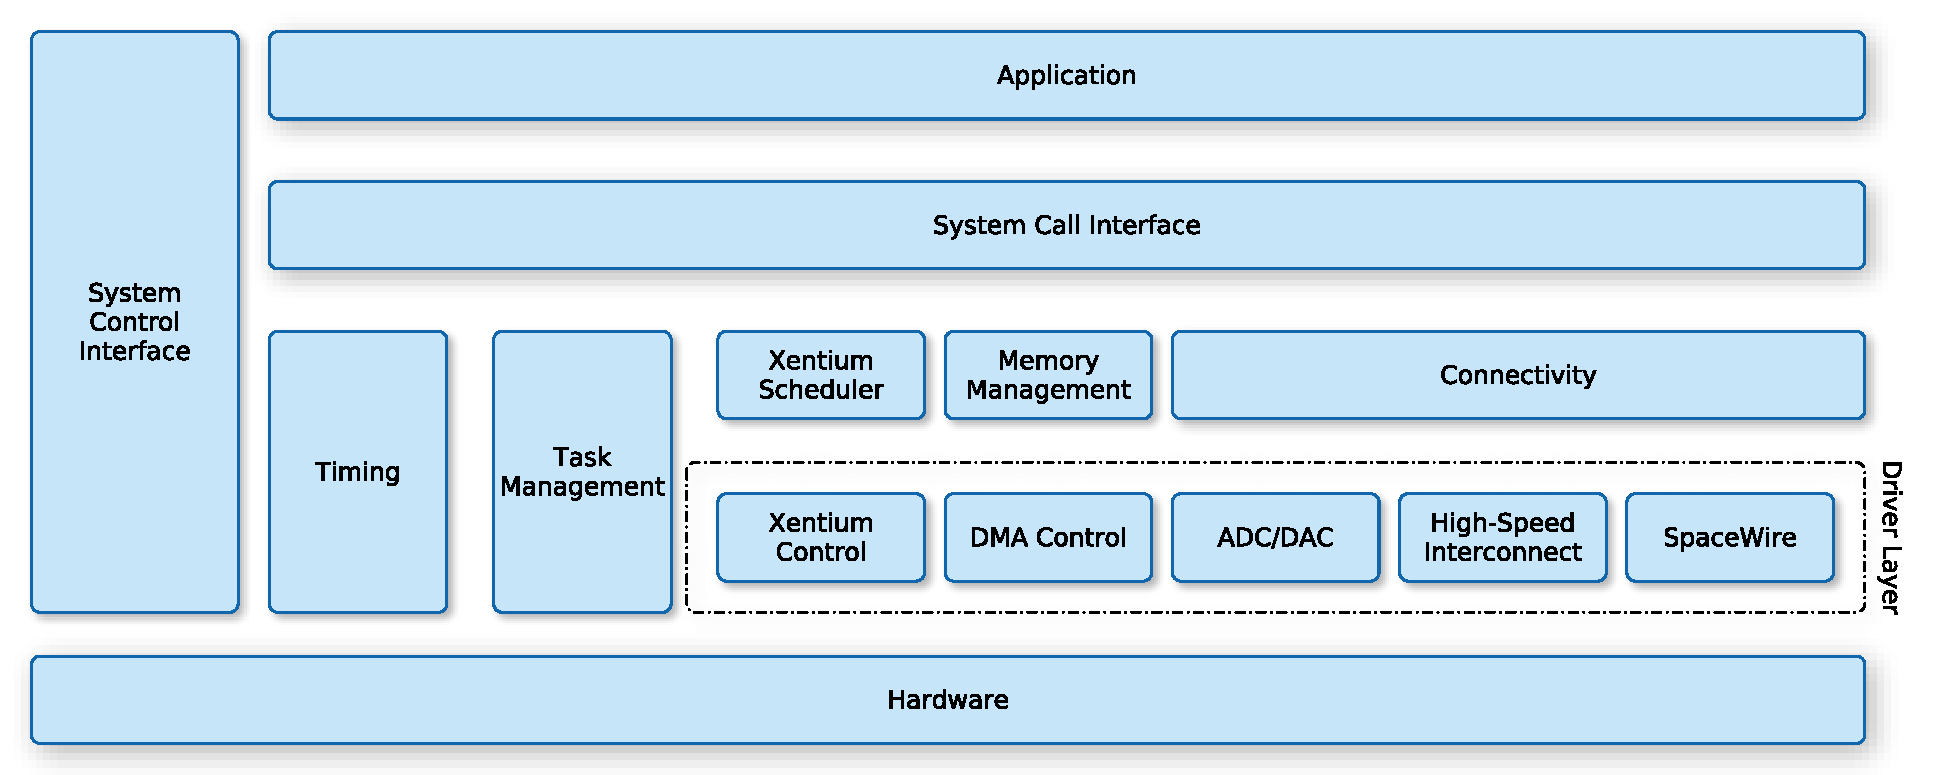
\includegraphics[width=\columnwidth]{../requirements/images/OS_logical}
	\caption{The architectural model of FlightOS. Here, the "hardware" layer
	represents both the hardware and the hardware abstraction layer of
	the software.}
	\label{fig:logical_model}
\end{center}
\end{figure}


In FlightOS, the \gls{SSDP} hardware is accessed in multiple layers of
abstraction (see \fig{fig:logical_model}). Typical \gls{CPU} tasks such as
thread/task management and timer operation are used as part of the operating
system kernel and are also accessible by user applications via a system call
interface. Other functional hardware components of the \gls{SSDP} such as the
\gls{NoC} \gls{DMA} have their own driver modules. These are in turn used by the
\gls{Xentium} scheduler and other higher level modules in the operating system.
Configuration of and access to the latter from user space is done via a system
call interface. The system control interface serves as an intermediate between
all layers of the operating system, where system or module states and hardware
modes or usage statistics may be exported by individual components for external
(user) access.




\section{Software Components Design - General}


\design{GEN-0001}%
{Boot}{%
This is the hardware entry point of FlightOS. The boot procedure sets up and
configures the \gls{LEON3-FT} processor for operation, initialises a minimum set of 
needed hardware devices and memories as well as the initial system stack.
}%
{\meetsreq{GEN-0006, FUN-0007, FUN-0804}}{}



\design{GEN-0002}
{User Space}{%
After the kernel has finished initialising, it calls a function
\mbox{\emph{kernel\_init()}}
that executes an \emph{init()} function configured by the user. This is the
run-time adaptation point from which user space is started. From there, the user
can start processes and reconfigure or load kernel options and modules via the
system call or sysctl interfaces.
}%
{\meetsreq{FUN-0804}}{}



\design{GEN-0003}%
{Interrupts, Traps}
{In order to operate a \gls{SPARC} v8 \gls{CPU} properly, a trap table must be
configured, in particular to handle register window under and overflow traps if
used with regular \gls{GCC} code generation for the target platform.
FlightOS configures a callback system for interrupt traps that can later be used
to install custom handlers, for example as part of driver modules.\newline

Interrupt statistics are exported via the system control interface.
}%
{\meetsreq{GEN-0006, GEN-0009, GEN-0018, GEN-0010, FUN-0023}}%
{The trap table and its function are described in \cite{SPARCv8} in detail.}



\design{GEN-0004}%
{Timers}{%
Timing functionality is a core element of an operating system by scheduling
periodic and non-periodic kernel wakeup events that subsequently control the
system's exectuion. The operating system kernel maintains these timers to
measure time or schedule kernel wakeups.

In addition to the \gls{CPU} bound timers, the real-time clock of the \gls{SSDP}
is supported.
}%
{\meetsreq{FUN-0011, FUN-0016, FUN-0017}}{}


\design{GEN-0005}%
{Kernel Mode}{%
The operating system protects access to privileged registers by disabling
supervisor mode when switching to user space. On the \gls{SPARC}v8, traps enable
supervisor mode, so the privileged mode is automatically entered when the kernel
is executing after a trap/interrupt or a system call from user space, which is
also implemented via the trap table.\newline

Kernel and unmapped memory access from user space is protected by the \gls{MMU}.
}%
{\meetsreq{FUN-0803, FUN-0008}}{}


\design{GEN-0006}%
{\gls{MMU}}{%
The kernel uses the \gls{MMU} to map pages of the system memory into a virtual
address space for most of its own processes and for user space.

If needed, physical memory is directly accessible by driver components or
mapped accordingly.

}%
{\meetsreq{FUN-0803, FUN-0008}}{The proper handling of address space translation
is particularly relevant for use with the \gls{NoC} \gls{DMA} driver and
\gls{Xentium} scheduler.}



\design{GEN-0007}%
{Thread Support}{%
This component supports the definition and creation of tasks. Task priorities
and scheduling deadlines are supported depending on the selected mode.\newline

Synchronisation and execution control between threads is provided via semaphores
and mutexes.
}%
{\meetsreq{FUN-0012, FUN-0013, FUN-0019}}{}


\design{GEN-0008}%
{Thread Scheduling}{%
Threads are scheduled by the kernel according to their run state, their
priorities and optionally their deadline.\newline

The state of mutexes and semaphores is used to temporarily re-order priorities if
needed, so lower priority threads do not block higher priority threads and vice
versa when locks are employed.\newline

Unless strict \gls{FIFO} mode is configured, threads of all scheduling
priorities are regularly assigned an execution time slice. The length of this
time slice decreases with priority. If \gls{gls-RR} scheduling is to be used,
time slices are set to be equal for all threads regardless of priority.
The latter is then only used to control re-ordering of the thread schedule to
more efficiently solve mutex lock situations. The user is in any case
responsible to assign different priorities to threads where deadlock situations
might occur that cannot be resolved by the scheduler (e.g. with identical
priorities).\newline

Access to mutexes and semaphores result in random scheduling events if the lock
is actively held or waited for by any other threads.
In tickless mode, regular scheduling occurs when a thread is preempted at the
end of its timeslice.\newline

If the kernel is configured to tick periodically, scheduling events will occur
at a configurable integer fraction of that rate.\newline

A special type of real-time thread is supported, which, with the exception of
an \gls{ISR} may also preempt the operating system kernel if its release
condition occurs and may run to its deadline without being preempted by other
threads. This functionality is reserved for highly timing-critical tasks and 
is reserved to functionality and modules executed in kernel space.\newline


If a multi-core processor is present in the system, the kernel can schedule
tasks to run on more than one \gls{CPU} if so configured.

}%
{\meetsreq{FUN-0014, FUN-0015, FUN-0016, FUN-0017, FUN-0019, FUN-0020, GEN-0028}}{}


\design{GEN-0009}%
{Message Queues}{%
Message queues are a facility for tasks/processes to communicate arbitrary 
data to each other. A named queue is created by one thread and opened by at
least one other thread. The threads can then send and receive messages
of arbitrary length. If a thread wants to actively wait for a message, it can
request to be notified and is subsequently woken by the scheduler once a message
arrives.
}%
{\meetsreq{FUN-0021}}{The implementation follows the \gls{POSIX} message
queue \gls{API} definition.}


\design{GEN-0010}%
{Loadable Modules}{%
Kernel modules can be loaded via the system call interface. The module is
supplied as an \gls{ELF} binary that holds special sections that are executed
by the kernel as their \emph{init()} or \emph{exit()} functions whenever
they are loaded or unloaded. \newline

The \emph{init} function of a module is typically
used to configure its functionality within the kernel, e.g. register a
thread, gain access to a hardware device or register an interrupt callback.
If the module is no longer needed or explicitly unloaded by the user, the
\emph{exit} function is used to de-register and clean up functionality
used by the module. \newline

Start-up arguments can be supplied to the module during loading. At run time,
the module may publish its internal settings via the kernel's system control
interface.
}%
{\meetsreq{FUN-0022}}{}


\design{GEN-0011}%
{System Control Interface}{%
The system control interface is a generic parseable interface that is accessible
from user and kernel space. It is modeled on a logical tree that holds nodes
representing entries of kernel components and can be viewed as a file/directory
structure. The input/output of each entry and how it may be parsed is defined
by its creator and may be used for run-time configuration or statistics keeping.
\newline

Data may be read and written to the nodes and are exchanged via
character-based text.\newline

Special nodes may be created that allow exchange of raw binary data, for example
internal memory dumps or configuration data.\newline

The entries in a node are functions that are part of a module or system
component. The component registers these functions along with a name and a
positional branch name within the logical tree. Components may also define new
branches where their interface is positioned.\newline

If the node is read, the system control interface executes the associated
output function of the component and returns a character buffer to the reader.
\newline

If the node is written, the writer-supplied buffer is passed to the component's
internal associated input function and parsed by the latter. \newline

Success or failure of the operation depends on the correct use of the individual
make-up of the character buffers.
}%
{\meetsreq{FUN-0023, FUN-0024}}{}


\design{GEN-0012}%
{\gls{SpaceWire} Driver}{%
The \gls{SpaceWire} devices of the \gls{SSDP} are accessible from user space via
a file descriptor that can be read or written atomically.
If a \gls{SpaceWire} device is only used in the \gls{Xentium} processing
network, it may be configured by the driver for direct \gls{DMA} to the input
buffer stage. Similarly, it may be used with \gls{DMA} for the output buffer
stage.

If the \gls{RMAP} feature is to be used, the configured physical memory block
is mapped into a virtual memory space.
}%
{\meetsreq{FUN-0025, FUN-0026, FUN-0027}}{}


\design{GEN-0013}%
{\gls{ADC}/\gls{DAC} Driver}{%
The \gls{ADC}/\gls{DAC} devices of the \gls{SSDP} are accessible from user
space via a file descriptor that can be read or written atomically.
If a \gls{ADC} device is only used in the \gls{Xentium} processing
network, it may be configured by the driver for direct \gls{DMA} to the input
buffer stage. Similarly, the \gls{DAC} may be used with \gls{DMA} for the
output of the processing chain.
}%
{\meetsreq{FUN-0025}}{}


\design{GEN-0014}%
{Xentium Driver}{%
The \gls{Xentium} driver and scheduler loads binary images of functional
\gls{DSP} program kernels via a system call interface. Each image is assigned a
signature that identifies the type of function of the \gls{DSP} kernel and a
mask that control the number of instances and \gls{Xentium} \glspl{DSP} it
may run on at any time. \newline

To each \gls{DSP} kernel image, an input buffer is assigned, which stores
references to metadata packets. Buffer fill level thresholds are defined that
control the dynamic processing priority during run-time. \newline

The first threshold defines the \emph{minimum} fill level above which the
processing kernel may be scheduled. This is relevant in situations where more
than input packets are needed to perform a task. \newline

The second threshold is the \emph{low} threshold.
As long as the buffer fill level is below this threshold, it is only scheduled
with the lowest priority. If the level is above the \emph{low} threshold, the
buffer contents are scheduled with \emph{medium} priority. \newline

The third threshold is the \emph{high} threshold. If the buffer level exceeds
this threshold, it is scheduled for processing with the highest priority.
}%
{\meetsreq{FUN-0026}}{%
The minimum input threshold is useful in situations where the processing kernel
must combine individual data segments, for example when stacking individual
frames that passed through preprocessing stages earlier.
}


\design{GEN-0015}%
{Xentium Queues}{%
The scheduling queues are ordered by buffer fill level. The queue is updated
as packets move between metadata buffers. The update mechanism is part of the
metadata buffers and triggers a message to the driver whenever a level threshold
is either over- or under-run and the most recent critical (\emph{high}) buffer is
moved to the head of the queue. If all buffers are above the \emph{high}
threshold, they are processed in an \gls{gls-RR} pattern. \newline

The driver maintains a separate \emph{bonded} queue for each \gls{DSP} that
holds program kernels that are allowed to run only on a particular \gls{DSP} and
one shared queue that holds all other kernels. The scheduling priority of
equal-level buffer states of bonded queues is higher than the shared queue,
i.e.\ buffers above the \emph{high} threshold in a bonded queue are processed
first, followed by the \emph{high} buffers in the shared queue, followed by the
\emph{medium} level buffers in the bonded queue etc.
}%
{\meetsreq{FUN-0027}}{}


\design{GEN-0016}%
{Xentium Scheduler}{%
If a program kernel's buffer is above the \emph{high} threshold, duplicates of
the program kernel may be scheduled to run in parallel on other \glspl{DSP}
according to the kernel's control mask. If more than two \glspl{Xentium} are
available in the system, the distribution scheduling algorithm ensures that 
all available \glspl{DSP} are assigned a program kernel above the \emph{high}
threshold with respect to their queues before scheduling duplicate instances.
If \glspl{DSP} are available, the head of the queue is duplicated according to
its control mask, followed by the next item and so on, as long as free
\glspl{Xentium} are available and pending \emph{high} threshold buffers exist
in the queue. \newline

The driver also maintains a special type of metadata buffer for input and output
nodes that connect the \gls{Xentium} processing chain to external data links
or mass storage. Of these, the input buffers are processed with the highest
absolute priority relative to their fill status. This is done to ensure that
if a data flow stall occurs, it does so as far back in the processing chain as
possible and data input is maintained until all buffers are filled to their
limit.
}%
{\meetsreq{FUN-0026, FUN-0027}}{%
Typically, the input buffer is the input for a special \gls{DSP} kernel
that processes and interprets the incoming data stream (of e.g. \gls{PUS} 
packets) and prepares and/or distributes metadata packets to the inputs of the
processing kernels according to the desired application.
}



\design{GEN-0017}%
{Xentium Data Buffers}{%
The metadata buffers track metadata packets as they move through the processing
network. With the exception of the input buffers to the network, they are
the input of one and the output of an arbitrary number of \gls{Xentium} program
kernels. Each item in a buffer corresponds to one metadata packet descriptor.
\newline

A metadata packet holds a pointer to data buffers of arbitrary size and a
field describing a route through the processing network of available kernels
by their signature identifier, i.e. it defines its own processing chain.
Each entry holds an associated pointer to an optional argument field, which may
hold parameters for the processing kernel. \newline

Program kernels may collect one or more of these packets at their input
depending on their processing functionality and either operate on the contents
of the packet or generate new packets from one or more input packets.
\newline

As the packet moves through the kernels, items on the processing routing 
stack are moved to a history field and they are output into a meta-buffer
according to their pending routing node.
}%
{\meetsreq{FUN-0027}}{}





\section{Software Components Design - Aspects of each Component}

The detailed design of the individual components is documented as part of 
their source code in Doxygen markup. This ensures continued flexibility in
development and allow for effortless maintainance of a fully update state
between the implementation and its detailed documentation.

\section{Internal Interface Design}

The internal interfaces of the operating system are described as part of the
source code in Doxygen markup and may be generated from there.

\section{Requirements to Design Components Traceability}

\noindent
Functional requirements are always reference to their design components, others
only as needed or for clarification. This is reflected in the traceability
matrix.

\traceabilitymatrix

\end{document}
